\chapter{Linear Algebra}\label{chapter:linear_algebra}

\section{Vector spaces}

    \newdef{$K$-vector space}{\index{vector!space}\label{linalgebra:vector_space}
        Let $K$ be a field. A $K$-vector space $V$ is a set equipped with two operations, \textbf{(vector) addition} $V\times V\rightarrow V$ and \textbf{scalar multiplication} $K\times V\rightarrow V$, that satisfy the following axioms:
        \begin{enumerate}
            \item $V$ forms an Abelian group under vector addition.
            \item Scalar multiplication is associative: $\lambda(\mu v) = (\lambda\mu)v$ for all $\lambda,\mu\in K$ and $v\in V$.
            \item The identity of the field $K$ acts as a neutral element for scalar multiplication: $1_Kv = v$ for all $v\in V$.
            \item Scalar multiplication is distributive with respect to vector addition: $\lambda(v+w) = \lambda v + \lambda w$ for all $\lambda\in K$ and $v,w\in V$.
            \item Vector addition is distributive with respect to scalar multiplication: $(\lambda+\kappa)v = \lambda v + \kappa w$ for all $\lambda,\kappa\in K$ and $v\in V$.
        \end{enumerate}
    }
    From here on the underlying field $K$ will be left implicit unless the results depend on it.

    \remark{The above definition can be restated in abstract algebraic terms. A $K$-vector space is a module (\cref{algebra:module}) over $K$.}

\subsection{Linear independence}

    \newdef{Linear combination}{\index{basis!Hamel}\label{linalgebra:linear_combination}
        The vector $w$ is a linear combination of elements in the set $\{v_i\}_{i\leq n}\subset V$ if it can be written as
        \begin{gather}
            w = \sum_{i=1}^n\lambda_iv_i
        \end{gather}
        for some $\{\lambda_i\}_{i\leq n}\subset K$. One can generalize this to general subsets $S\subseteq V$, but the number of nonzero elements $\lambda_i$ is always required to be finite.\footnote{Generalizations are possible in the context of topological vector spaces (see \cref{chapter:topology} and \cref{chapter:functional}), where one can define the notion of convergence.} (See \cref{linalgebra:hamel_remark} about \textit{Hamel bases}.)
    }
    \newdef{Linear independence}{\label{linalgebra:linear_independence}
        A finite set $\{v_i\}_{i\leq n}$ is said to be linearly independent if the following relation holds:
        \begin{gather}
            \sum_{i=1}^n\lambda_i v_i = 0 \iff \forall i\leq n:\lambda_i = 0\,.
        \end{gather}
        A general set $S\subset V$ is said to be linearly independent if every finite subset of it is linearly independent.
    }

    \newdef{Span}{\index{span}
        A set of vectors $S\subseteq V$ is said to span $V$ if every vector $v\in V$ can be written as a linear combination of elements in $S$.
    }

    \newdef{Frame}{\index{frame}\label{linalgebra:frame}
        A $k$-frame is an ordered set of $k$ linearly independent vectors.
    }

\subsection{Bases}\index{basis}

    \newdef{Basis}{
        A subset $\mathcal{B}\subset V$ that is linearly independent and spans $V$.
    }
    \begin{property}
        Every spanning set contains a basis.
    \end{property}

    \begin{remark}[Hamel basis]\index{basis!Schauder}\index{basis!Hamel}\label{linalgebra:hamel_remark}
        In the previous definition, the concept of a Hamel basis was implicitly used. This concept is based on two conditions:
        \begin{enumerate}
            \item The basis is linearly independent.
            \item Every element in the vector space can be written as a linear combination of a \underline{finite} subset of the basis.
        \end{enumerate}
        For bases consisting of a finite number of vectors, one does not have to worry. However, for infinite bases one has to keep this in mind. An alternative construction that allows for combinations of a countably infinite number of elements, is given by that of a \textit{Schauder basis}.
    \end{remark}
    Nonetheless, it can be shown that every vector space admits a Hamel basis.
    \begin{construct}[\difficult{Hamel basis}]\index{basis!Hamel}\label{linalgebra:hamel_basis}
        Let $V$ be a vector space and consider the set of all linearly independent subsets of $V$. Under the relation of inclusion this set becomes a partially ordered set (\cref{set:poset}). Zorn's lemma~\ref{set:zorns_lemma} then says that there exists at least one maximal linearly independent set.

        Now, one can show that this maximal subset $S$ is also a spanning set of $V$. Choose a vector $v\in V$ that is not already in $S$. From the maximality of $S$ it follows that $S\cup v$ is linearly dependent and, hence, there exists a finite sequence of scalars $(a^1,\ldots,a^n,b)$ and a finite sequence of elements $(e_1,\ldots,e_n)$ in $S$ such that:
        \begin{gather}
            \sum_{i=0}^n a^ie_i + bv = 0\,,
        \end{gather}
        where not all scalars are zero. This implies that $b\neq0$, because otherwise the set $\{e_i\}_{i\leq n}$ and, hence, also $S$ would be linearly dependent. It follows that $v$ can be written as\footnote{It is this step that requires $R$ to be a division ring in \cref{algebra:module_basis} because otherwise one would in general not be able to divide by $b\in R$.}
        \begin{gather}
            v = -\frac{1}{b}\sum_{i=0}^na^ie_i\,.
        \end{gather}
        Because $v$ was chosen randomly, one can conclude that $S$ is a spanning set for $V$.
    \end{construct}
    \begin{remark*}
        This construction assumes the axiom of choice in set theory, only ZF does not suffice. It can even be shown that the existence of a Hamel basis for every vector space is equivalent to the axiom of choice.
    \end{remark*}

    \begin{property}
        Every basis of a vector space has the same number of elements. For infinite-dimensional spaces this means that all bases have the same \textit{cardinality}.
    \end{property}
    \newdef{Dimension}{\index{dimension!of vector space}\label{linalgebra:dimension}
        Let $V$ be a finite-dimensional vector space and let $\mathcal{B}$ be a basis for $V$ with $n$ elements. With the previous property in mind, the dimension of $V$ is defined as follows:
        \begin{gather}
            \dim(V) := n\,.
        \end{gather}
    }

    \newdef{Subspace}{\label{linalgebra:subspace}
        Let $V$ be a vector space. A subset $W$ of $V$ is called a subspace if $W$ is itself a vector space under (the restriction of) the operations of $V$:
        \begin{gather}
            W\leq V\iff\forall w_1,w_2\in W,\forall\lambda\in K:\lambda w_1 + w_2 \in W\,.
        \end{gather}
    }

\subsection{Sum and direct sum}

    \newdef{Sum}{\index{sum}
        \nomenclature[O_zsymbinsum]{$X+Y$}{sum of the vector spaces $X$ and $Y$}
        Let $V$ be a vector space and consider a finite collection of subspaces $\{W_1,\ldots,W_k\}$. The sum of these subspaces is defined as follows:
        \begin{gather}
            W_1+\cdots+W_k := \left\{\sum_{i=1}^kw_i\,\middle\vert\,w_i\in W_i\right\}\,.
        \end{gather}
        For an infinite collection of subspaces the linear combinations have to be finite.
    }
    \newdef{Direct sum}{\index{direct!sum}\label{linalgebra:direct_sum}
        \nomenclature[O_zsymbinsump]{$X\oplus Y$}{direct sum of the vector spaces $X$ and $Y$}
        If every element $v$ of the sum can be written as a unique linear combination, the sum is called a direct sum.
    }
    \newnot{Direct sum}{
        The direct sum of vector spaces is denoted by
        \begin{gather*}
            W_1\oplus\cdots\oplus W_k\equiv\bigoplus_{i=1}^kW_i\,.
        \end{gather*}
    }

    \begin{formula}
        Let $V$ be a finite-dimensional vector space and consider two subspaces $W_1,W_2\leq V$. The dimensions of these spaces can be related in the following way:
        \begin{gather}
            \dim(W_1+W_2) = \dim(W_1) + \dim(W_2) - \dim(W_1\cap W_2)\,.
        \end{gather}
    \end{formula}
    \begin{property}
        Let $V$ be a vector space and assume that $V$ can be decomposed as $W=W_1\oplus W_2$. If $\mathcal{B}_1$ is a basis of $W_1$ and if $\mathcal{B}_2$ is a basis of $W_2$, then $\mathcal{B}_1\cup\mathcal{B}_2$ is a basis of $W$.
    \end{property}

    \newdef{Complement}{\index{complement!vector space}
        Let $V$ be a vector space and let $W$ be a subspace of $V$. A subspace $W'$ of $V$ is called a complement of $W$ if $V = W\oplus W'$.
    }
    \begin{property}[Existence of complements]\label{linalgebra:complement}
        Let $V$ be a vector space and let $U,W$ be two subspaces of $V$. If $V = U+W$, there exists a subspace $Y\leq U$ such that $V = Y\oplus W$. In particular, every subspace of $V$ has a complement in $V$.
    \end{property}

\section{Linear maps}

    \newdef{Linear map}{\index{linear!map}
        Let $V,W$ be $K$-vector spaces. A function $f:V\rightarrow W$ is said to be linear if $f(\lambda v+w)=\lambda f(v)+f(w)$ for all $\lambda\in K$ and $v,w\in V$.
    }

    \remark{Linear maps are also called \textbf{linear transformations} or \textbf{linear mappings}.}

\subsection{Homomorphisms}

    \newdef{Homomorphism space}{\index{morphism!of vector spaces}\label{linalgebra:hom_space}
        \nomenclature[S_VectK]{$\mathbf{Vect}_K$}{category of vector spaces and linear maps over a field $K$}
        Let $V,W$ be two vector spaces. The set of all linear maps between $V$ and $W$ is called the homomorphism space from $V$ to $W$:
        \begin{gather}
            \hom_K(V,W) := \bigl\{f:V\rightarrow W\bigm\vert f\text{ is linear}\bigr\}\,.
        \end{gather}
        The collection of $K$-vector spaces and linear maps between them form a category $\mathbf{Vect}_K$.
    }
    \begin{formula}\label{linalgebra:hom_dimension}
        Let $V,W$ be two finite-dimensional vector spaces.
        \begin{gather}
            \dim\bigl(\hom_K(V,W)\bigr) =\dim(V)\dim(W)
        \end{gather}
    \end{formula}

    \newdef{Endomorphism ring}{\index{endo-!morphism}
        The space $\hom_K(V,V)$ with composition of maps as multiplication forms a ring, the endomorphism ring. It is denoted by $\End_K(V)$ or $\End(V)$ when the underlying field is clear.
    }
    \begin{property}[Commutator]\index{commutator}
        The endomorphism ring $\End(V)$ can also be endowed with the structure of a \textit{Lie algebra} (see \cref{lie:end_as_lie_algebra}) by equipping it with the commutator
        \begin{gather}
            [A,B] := A\circ B - B\circ A\,.
        \end{gather}
    \end{property}

    \begin{property}
        Let $V$ be finite-dimensional vector space and let $f:V\rightarrow V$ be an endomorphism. The following statements are equivalent:
        \begin{itemize}
            \item $f$ is injective,
            \item $f$ is surjective, and
            \item $f$ is bijective.
        \end{itemize}
    \end{property}

    \newdef{Automorphism}{\index{automorphism}\index{general linear group}\label{linalgebra:automorphism}
        \nomenclature[S_GL]{$\GL(V)$}{general linear group, the group of automorphisms of a vector space $V$}
        An isomorphism from $V$ to $V$ is called an automorphism. The set of all automorphisms  on $V$ is denoted by $\Aut(V)$. It forms a group under composition. Often this group is called the general linear group\footnote{It is isomorphic to the general linear group of invertible \textit{matrices} (see \cref{linalgebra:GL_matrices}), hence the similar name and notation.} $\GL_K(V)$ or $\GL(V)$ when the underlying field is clear.
    }
    \remark{Sometimes automorphisms are also called \textbf{linear operators}. However, this terminology is also used for a general linear map in operator theory (\cref{chapter:operator_algebras}) and so this terminology is not adopted in this text.\index{operator}}

    \newdef{Kernel}{\index{kernel}
        Consider a linear map $f:V\rightarrow W$. The kernel of $f$ is defined as the following subspace of $V$:
        \begin{gather}
            \ker(f) := \{v\in V\mid f(v) = 0\}\,.
        \end{gather}
    }
    \begin{property}
        A linear map $f:V\rightarrow W$ is injective if and only if $\ker(f)=0$.
    \end{property}

    \newdef{Rank}{\index{rank!of a linear map}\label{linalgebra:image_rank}
        The dimension of the image of a linear map.
    }
    \newdef{Nullity}{\index{nullity}
        The dimension of the kernel of a linear map.
    }

    \begin{theorem}[Dimension theorem\footnotemark]\index{rank-nullity theorem}\label{linalgebra:dimension_theorem}
        \footnotetext{Also called the \textbf{rank-nullity theorem}.}
        Let $f:V\rightarrow W$ be a linear map.
        \begin{gather}
            \dim(\im(f)) + \dim(\ker(f)) = \dim(V)
        \end{gather}
    \end{theorem}
    \begin{result}\label{linalgebra:dimension_isomorphism}
        Two finite-dimensional vector spaces are isomorphic if and only if they have the same dimension.
    \end{result}

    \begin{property}[Jordan--Chevalley decomposition]\index{Jordan--Chevalley decomposition}\index{semisimple!operator}\index{nilpotent}\label{linalgebra:jordan_chevalley}
        Every endomorphism $A$ can be decomposed as follows:
        \begin{gather}
            A = A_{ss} + A_n\,,
        \end{gather}
        where
        \begin{itemize}
            \item $A_{ss}$ is \textbf{semisimple}: for every invariant subspace of $A_{ss}$ there exists an invariant complementary subspace.
            \item $A_n$ is \textbf{nilpotent}: $\exists k\in\mathbb{N}:A_n^k = 0$.
        \end{itemize}
        Furthermore, this decomposition is unique and the endomorphisms $A_{ss},A_n$ can be written as polynomials in $A$.
    \end{property}

\subsection{Dual maps}

    \newdef{Dual space}{\index{dual!space}\index{linear!form}\index{functional}\label{linalgebra:dual_space}
        Let $V$ be a vector space. The (algebraic) dual $V^*$ of $V$ is defined as the following vector space:
        \begin{gather}
            V^*:=\hom_K(V,K)=\bigl\{f:V\rightarrow K\bigm\vert f\text{ is linear}\bigr\}\,.
        \end{gather}
        The elements of $V^*$ are called \textbf{linear forms} or (linear) \textbf{functionals}.
    }
    \begin{property}[Dimension]\label{linalgebra:dual_space_dimension}
        From \cref{linalgebra:hom_dimension} it follows that $\dim(V^*)=\dim(V)$ whenever $V$ is finite-dimensional. If $V$ is infinite-dimensional, this property is \underline{never} valid. In the infinite-dimensional case $\mathrm{card}(V^*)>\mathrm{card}(V)$ always holds.
    \end{property}

    \newdef{Dual basis}{\index{basis!dual}\label{linalgebra:dual_basis}
        Let $\mathcal{B}=\{e_1,e_2,\ldots,e_n\}$ be a basis for a finite-dimensional vector space $V$. One can construct a basis $\mathcal{B}^*=\{\varepsilon_1,\varepsilon_2,\ldots,\varepsilon_n\}$ for $V^*$, called the dual basis of $\mathcal{B}$, as follows:
        \begin{gather}
            \varepsilon_i:\sum_{j=1}^na_ie_i\mapsto a_i\,.
        \end{gather}
        The relation between a basis and its associated dual basis can also be expressed as
        \begin{gather}
            \label{linalgebra:dual_basis_2}
            \varepsilon^i(e_j) = \delta^i_j\,.
        \end{gather}
    }
    \newdef{Natural pairing}{\index{natural!pairing}\label{linalgebra:natural_pairing}
        The definition of the dual basis extends to a natural pairing of $V$ and its dual $V^*$ in terms of the following bilinear map:
        \begin{gather}
            \langle v,v^* \rangle := v^*(v)\,.
        \end{gather}
        (See \cref{hda:dual} for a generalization of this map.)
    }

    \newdef{Dual map}{\index{dual!map}\index{transpose}\label{linalgebra:transpose}
        Let $f:V\rightarrow W$ be a linear map. The linear map
        \begin{gather}
            f^*:W^*\rightarrow V^*:\varphi\rightarrow\varphi\circ f
        \end{gather}
        is called the dual map or \textbf{transpose} of $f$. It is also often denoted by $f^T$.
    }
\section{Inner product}\label{section:innerproduct}

    In this section all vector spaces $V$ will be defined over $\mathbb{R}$ or $\mathbb{C}$.

\subsection{Inner product space}

    \newdef{Inner product}{\index{inner!product}\label{linalgebra:innerproduct}
        A function $\langle\cdot|\cdot\rangle:V\times V\rightarrow\mathbb{C}$ is called an inner product on $V$ if it satisfies the following properties for all $u,v,w\in V$ and $\lambda\in\mathbb{C}$:
        \begin{enumerate}
            \item\textbf{Conjugate symmetry}: $\langle v|w \rangle = \langle w|v \rangle^*$,
            \item\textbf{Linearity in the second argument}: $\langle u|\lambda v+w \rangle = \lambda\langle u|v \rangle + \langle u|w \rangle$,
            \item\textbf{Nondegeneracy}: $\langle v|v \rangle = 0 \iff v = 0$, and
            \item\textbf{Positive-definiteness}: $\langle v|v \rangle \geq 0$.
        \end{enumerate}
    }
    \begin{result}\index{sesquilinear}
        The first two properties have the result of conjugate linearity in the first argument:
        \begin{gather}
            \langle \lambda f + \mu g|h \rangle = \overline{\lambda}\langle f|h \rangle + \overline{\mu}\langle g|h \rangle
        \end{gather}
        Therefore, these two properties together are often combined into a \textbf{sesquilinearity} axiom. When the underlying field is restricted to $\mathbb{R}$, such that the conjugate symmetry property is replaced by proper symmetry, the inner product becomes a bilinear form.
    \end{result}

    \newdef{Inner product space}{\index{Hilbert!space}
        A vector space equipped with an inner product $\langle\cdot|\cdot\rangle$. This is sometimes called a \textbf{pre-Hilbert space}.
    }

    \newdef{Metric dual}{\label{linalgebra:metric_dual}
        Using the inner product (or any other nondegenerate Hermitian form) one can define the metric dual of a vector by the following map:
        \begin{gather}
            L:V\rightarrow V^*:v\mapsto\langle v|\cdot \rangle.
        \end{gather}
        (See Equation \eqref{riemann:flat_map} for a generalization.) If the sesquilinearity condition would have been stated in the reversed convention, i.e.~conjugate linearity in the second argument, metric duals would be conjugate linear and, hence, would not be proper elements of the dual space.
    }
    \newdef{Adjoint map}{\index{adjoint!Hermitian}\index{Hermitian}\index{self-adjoint}\label{linalgebra:adjoint_operator}
        Let $A$ be a linear map on $V$. The (\textbf{Hermitian}) adjoint of $A$ is defined as the linear map $A^\dag$ that satisfies
        \begin{gather}
            \langle A^\dag v|w\rangle = \langle v|Aw\rangle
        \end{gather}
        for all $v,w\in V$. Alternatively, one can define the adjoint using the transpose and metric dual as follows:
        \begin{gather}
            A^\dag = L^{-1}\circ A^*\circ L.
        \end{gather}
        If $A=A^\dag$, $A$ is said to be \textbf{Hermitian} or \textbf{self-adjoint}. (In Chapter \ref{chapter:functional} a distinction will be made between these two notions.)
    }

\subsection{Orthogonality}\label{section:orthogonality}

    \newdef{Orthogonal}{\index{orthogonal}\label{linalgebra:orthogonal}
        Consider two vectors $v,w\in V$ in an inner product space. These vectors are said to be orthogonal, denoted by $v\perp w$,  if they obey the following relation:
        \begin{gather}
            \langle v\mid w \rangle = 0.
        \end{gather}
        An \textbf{orthogonal system} is a collection of vectors, none of them equal to 0, that are mutually orthogonal.
    }
    \begin{property}
        Orthogonal systems are linearly independent.
    \end{property}

    \newdef{Orthonormal}{\index{orthonormal}\label{linalgebra:orthonormal}
        A set of vectors $S$ is said to be orthonormal if it forms an orthogonal system and if all the elements $v\in S$ obey the following relation:
        \begin{gather}
            \langle v\mid v \rangle = 1.
        \end{gather}
    }
    \newdef{Orthogonal complement}{\index{complement!vector space}\label{linalgebra:orthogonal_complement}
        Let $W$ be a subspace of an inner product space $V$. The orthogonal complement of $W$ is defined as the following subspace:
        \begin{gather}
            W^\perp := \{v\in V\mid\forall w\in W:\langle v\mid w\rangle = 0\}.
        \end{gather}
    }
    \sremark{$W^\perp$ is pronounced as ``W-perp''.}

    \begin{property}[Complements]
        Let $V$ be a finite-dimensional inner product space. The orthogonal complement $W^\perp$ is a complementary subspace to $W$, i.e.~$W\oplus W^\perp=V$.
    \end{property}
    \begin{result}\label{linalgebra:perp_of_perp}
        Let $W\leq V$ with $V$ a finite-dimensional inner product vector space. Forming orthogonal complements defines an involution:
        \begin{gather}
            (W^\perp)^\perp = W.
        \end{gather}
    \end{result}

    \newdef{Orthogonal projection}{\index{projection!orthogonal}\label{linalgebra:orthogonal_projection}
        Let $V$ be a finite-dimensional inner product vector space and consider a subspace $W\leq V$. Consider a vector $w\in W$ and let $\{w_1,\ldots,w_k\}$ be an orthonormal basis of $W$. The projections of $v\in V$ on $W$ and $w\in W$ are defined as follows:
        \begin{align}
            \proj_W(v) &:= \sum_{i=1}^k\langle v\mid w_i \rangle w_i\\
            \proj_w(v) &:= \frac{\langle v\mid w \rangle}{\langle w\mid w \rangle}w.
        \end{align}
    }
    \begin{property}
        Orthogonal projections satisfy the following conditions:
        \begin{gather}
            \forall w\in W:\proj_W(w) = w \qquad\text{and}\qquad \forall u\in W^\perp:\proj_W(u) = 0.
        \end{gather}
    \end{property}

    \newmethod{Gram-Schmidt orthonormalization}{\label{linalgebra:gram_schmidt}
        Let $\{u_i\}_{i\leq n}$ be a set of linearly independent vectors. An orthonormal set $\{e_i\}_{i\leq n}$ can be constructed out of $\{u_i\}_{i\leq n}$ using the following procedure:
        \begin{enumerate}
            \item Orthogonalization:
                \begin{gather}
                    \begin{aligned}
                        w_1& = u_1&\\
                        w_2& = u_2 - \frac{\langle u_2\mid w_1\rangle}{\|u_2\|^2}w_1&\\
                        &\vdots&\\
                        w_n& = u_n - \sum_{i=1}^{n-1}\frac{\langle u_n\mid w_i\rangle}{\|u_n\|^2}w_i&
                    \end{aligned}
                \end{gather}
            \item Normalization:
                \begin{gather}
                    \begin{aligned}
                        e_1& = \frac{w_1}{\|w_1\|}&\\
                        e_2& = \frac{w_2}{\|w_2\|}&\\
                        &\vdots&\\
                        e_n& = \frac{w_n}{\|w_n\|}&
                    \end{aligned}
                \end{gather}
        \end{enumerate}
    }
    \begin{remark}\index{Hermitian!form}\index{signature}\index{Lorentz!metric}\label{linalgebra:NDH_form}
        Inner products can be generalized to \textbf{nondegenerate Hermitian forms} which do not satisfy the positive-definiteness property. For any vector space with a nondegenerate Hermitian form, one can find a basis such $\{e_1,\ldots,e_{p+q}\}$ such that
        \begin{gather}
            \langle e_i\mid e_i \rangle=
            \begin{cases}
                1&i\leq p\\
                -1&p<i\leq p+q.
            \end{cases}
        \end{gather}
        These spaces are said to have (metric) \textbf{signature} $(p,q)$. A vector space with signature $(1,k)$ or $(k,1)$ is said to be \textbf{Lorentzian}. Note that the signature is basisindependent due to \textit{Sylvester's theorem} \ref{linalgebra:sylvester}.
    \end{remark}

    \newdef{Householder transformation}{\index{Householder transformation}\label{linalgebra:householder_transformation}
        Let $v$ be an element of an inner product space $V$. The Householder transformation generated by $v$ is defined as the linear map
        \begin{gather}
            \sigma_v:V\rightarrow V:w\mapsto w - 2\frac{\langle w\mid v \rangle}{\langle v\mid v \rangle}v.
        \end{gather}
        This transformation amounts to a reflection in the hyperplane orthogonal to $v$.
    }

    \newdef{Angle}{\index{angle}\label{linalgebra:angle}
        \nomenclature[O_zsymangle]{$\sphericalangle(\cdot,\cdot)$}{angle between two vectors}
        Let $v,w$ be elements of an inner product space $V$. The angle $\theta$ between $v$ and $w$ is defined by the following formula:
        \begin{gather}
            \cos\theta := \frac{\langle v\mid w \rangle}{\|v\|\|w\|}.
        \end{gather}
        The angle between two vectors $v,w$ is sometimes denoted by $\sphericalangle(v,w)$.
    }
\section{Matrices}

    \begin{notation}\label{linalgebra:matrix_set}
        The vector space of all $m\times n$-matrices defined over the field $K$ is denoted by $M_{m,n}(K)$. If $m=n$, the space is denoted by $M_n(K)$ or $M(n,K)$.
    \end{notation}

    \begin{property}[Dimension]\index{dimension!of matrix}\label{linalgebra:dimension_of_matrix_space}
        The dimension of $M_{m,n}(K)$ is $mn$.
    \end{property}

    \newdef{General linear group}{\index{general linear group}\label{linalgebra:GL_matrices}
        \nomenclature[S_GLn]{$\GL(n,K)$}{general linear group: the group of all invertible $n\times n$-matrices over the field $K$}
        The set of invertible matrices is called the general linear group and is denoted by $\GL_n(K)$ or $\GL(n,K)$.
    }
    \begin{property}
        For all $A\in\GL_n(K)$ one has:
        \begin{itemize}
            \item $A^T\in\GL_n(K)$, and
            \item $\left(A^T\right)^{-1}=\left(A^{-1}\right)^T$.
        \end{itemize}
    \end{property}

    \newdef{Trace}{\index{trace}\label{linalgebra:trace}
        Let $A\equiv(a_{ij})\in M_n(K)$. The trace of $A$ is defined as follows:
        \begin{gather}
            \tr(A) := \sum_{i=1}^na_{ii}\,.
        \end{gather}
    }
    \begin{property}\label{linalgebra:trace_commutative}
        Let $A,B\in M_n(K)$. The trace satisfies the following properties:
        \begin{itemize}
            \item $\tr:M_n(K)\rightarrow K$ is a linear map,
            \item $\tr(AB) = \tr(BA)$, and
            \item $\tr(A^T) = \tr(A)$.
        \end{itemize}
    \end{property}

    \newformula{Hilbert--Schmidt norm}{\index{Frobenius!norm|see{Hilbert--Schmidt}}\index{Hilbert--Schmidt!norm}\label{linalgebra:hilbert_schmidt_norm}
        The Hilbert--Schmidt (or \textbf{Frobenius}) norm is defined by the following formula:
        \begin{gather}
            \|A\|^2_{HS} := \sum_{i,j}|A_{ij}|^2 = \tr\left(A^\dag A\right)\,.
        \end{gather}
        If one identifies $M_{n}(\mathbb{C})$ with $\mathbb{C}^{2n}$, this norm equals the standard Hermitian norm.
    }

    \newformula{Hadamard product}{\index{Hadamard!product}\label{linalgebra:hadamard_product}
        The Hadamard product of two matrices is defined as the entrywise product:
        \begin{gather}
            (A\circ B)_{ij} := A_{ij}B_{ij}\,.
        \end{gather}
    }

    \begin{property}\label{linalgebra:dim_columns_rows}
        Let $A\in M_{m,n}(K)$. Denote the set of columns as $\{A_1,A_2,\ldots,A_n\}$ and the set of rows as $\{R_1,R_2,\ldots,R_m\}$. The set of columns is a subspace of $K^m$ and the set of rows is a subspace of $K^n$. Their spans satisfy the following property:
        \begin{gather}
            \dim(\mathrm{span}(A_1,\ldots,A_n)) = \dim(\mathrm{span}(R_1,\ldots,R_m))\,.
        \end{gather}
    \end{property}
    \newdef{Rank}{\index{rank!of a matrix}\label{linalgebra:matrix_rank}
        Using the invariance relation from the previous property, one can define the rank of a matrix $A\in M_{m,n}(K)$ as follows:
        \begin{gather}
            \rk(A) := \dim(\mathrm{span}(A_1,\ldots,A_n)) = \dim(\mathrm{span}(R_1,\ldots,R_m))\,.
        \end{gather}
    }

    \begin{property}\label{linalgebra:rank_properties}
        Let $A\in M_{m,n}(K),B\in\GL_n(K),C\in M_{n,r}(K)$ and $D\in M_{r,n}(K)$. The ranks of these matrices satisfy the following properties:
        \begin{itemize}
            \item $\rk(AC)\leq\rk(A)$,
            \item $\rk(AC)\leq\rk(C)$,
            \item $\rk(BC)=\rk(C)$, and
            \item $\rk(DB)=\rk(D)$.
        \end{itemize}
    \end{property}
    \begin{property}\label{linalgebra:matrix_left_multiplication}
        Let $A\in M_{m,n}(K)$. The linear map
        \begin{gather}
            L_A:K^n\rightarrow K^m:v\mapsto Av
        \end{gather}
        satisfies $\im(L_A)=\mathrm{span}(A_1,\ldots,A_n)$.
    \end{property}

\subsection{System of equations}\label{section:system_of_equations}

    \begin{property}\label{linalgebra:matrix_and_equations}
        Let $Ax=b$ with $A\in M_{m,n}(K),x\in K^n$ and $b\in K^m$ be a system of $m$ equations in $n$ variables and let $L_A$ be the linear map as defined in \cref{linalgebra:matrix_left_multiplication}. The following properties hold:
        \begin{itemize}
            \item The system is inconsistent if and only if $b\not\in\im(L_A)$.
            \item If the system is not inconsistent, the solution set is an affine space. If $x_0\in K^n$ is a solution, the solution set is given by: $x_0+\ker(L_A)$.
            \item If the system is homogeneous, i.e.~$b=0$, the solution set is equal to $\ker(L_A)$.
        \end{itemize}
    \end{property}
    \begin{property}[Uniqueness]\label{linalgebra:rank_unique_solution}
        Let $Ax=b$ with $A\in M_n(K)$ be a system of $n$ equations in $n$ variables. If $\rk(A)=n$, the system has a unique solution.
    \end{property}

    \newformula{Cramer's rule}{\index{Cramer's rule}\label{linalgebra:cramers_rule}
        Let $Ax=b$ be a system of linear equations where the matrix $A$ has a nonzero determinant. There exists a unique solution:
        \begin{gather}
            x_i = \frac{\det(A_i)}{\det(A)}\,,
        \end{gather}
        where $A_i$ is the matrix obtained by replacing the $i^{th}$ column of $A$ by the column vector $b$.
    }

\subsection{Coordinates and matrix representations}

    \newdef{Coordinate vector}{\index{coordinate}\label{linalgebra:coordinate_vector}
        Let $\mathcal{B}=\{b_1,\ldots,b_n\}$ be a basis of $V$ and consider the vector $v=\sum_{i=1}^n\lambda_ib_i$. The coordinate vector of $v$ with respect to $\mathcal{B}$ is defined as the column vector $(\lambda_1,\ldots,\lambda_n)^T$. The scalars $\lambda_i$ are called the \textbf{coordinates} of $v$ with respect to $\mathcal{B}$.
    }
    \newdef{Coordinate isomorphism}{\label{linalgebra:coordinate_isomorphism}
        With the previous definition in mind one can define the coordinate isomorphism induced by $\mathcal{B}$ as follows:
        \begin{gather}
            \beta:V\rightarrow K^n:\sum_{i=1}^n\lambda_ib_i\mapsto(\lambda_1,\ldots,\lambda_n)^T\,.
        \end{gather}
    }

    \begin{construct}[Matrix representation]\label{linalgebra:matrix_representation}
        Let $V,W$ be $m$- and $n$-dimensional vector spaces with bases $\mathcal{B}=\{b_1,\ldots,b_m\},\mathcal{C}=\{c_1,\ldots,c_n\}$ and consider a linear map $f:V\rightarrow W$. The matrix representation of $f$ with respect to $\mathcal{B}$ and $\mathcal{C}$ is defined as the matrix $A_{f,\mathcal{B},\mathcal{C}}$ that satisfies the following condition for all vectors $v\in V$. Let $(\lambda_1,\ldots,\lambda_n)^T$ be the coordinate vector of $v$ with respect to $\mathcal{B}$ and let $(\mu_1,\ldots,\mu_m)^T$ be the coordinate vector of $f(v)$ with respect to $\mathcal{C}$, then
        \begin{gather}
            \label{linalgebra:matrix_representation_equation}
            \begin{pmatrix}
                \mu_1\\\vdots\\\mu_m
            \end{pmatrix}
            = A_{f,\mathcal{B},\mathcal{C}}
            \begin{pmatrix}
                \lambda_1\\\vdots\\\lambda_n
            \end{pmatrix}\,.
        \end{gather}
        This matrix can be constructed as follows. For every $j\in\{1,\ldots,m\}$, write $f(b_j)=\sum_{i=1}^na_{ij}c_i$. The matrix $A_{f,\mathcal{B},\mathcal{C}}\equiv(a_{ij})\in M_{n,m}(K)$ is called the matrix representation of $f$. The $j^{th}$ column of $A_{f,\mathcal{B},\mathcal{C}}$ coincides with the coordinate vector of $f(b_j)$ with respect to $\mathcal{C}$.
    \end{construct}

    The following property shows that the matrix algebra $M_{m,n}(K)$ is isomorphic to the algebra\footnote{The multiplication is given by the composition of linear maps.} of linear maps $\mathcal{L}(K^n,K^m)$, thereby explaining why the same notation for the space of invertible matrices (\cref{linalgebra:GL_matrices}) and the space of automorphisms (\cref{linalgebra:automorphism}) was used.
    \begin{property}[Matrices and linear maps]\label{linalgebra:map_matrix_relation}
        For every matrix $A\in M_{m,n}(K)$ there exists a linear map $f:K^n\rightarrow K^m$ such that $A_{f,\mathcal{B},\mathcal{C}}=A$. Conversely, for every linear map $f:K^m\rightarrow K^n$ there exists a matrix $A\in M_{n,m}(K)$ such that $f=L_A$ (given by the previous construction).
    \end{property}
    \begin{result}\label{linalgebra:matrix_invertible_map}
        Let $f\in\End(V)$ and let $A_f$ be the corresponding matrix representation. The linear map $f$ is invertible if and only if $A_f$ is invertible. Furthermore, if $A_f$ is invertible,
        \begin{gather}
            \left(A_f\right)^{-1} = A_{f^{-1}}\,.
        \end{gather}
        In other words, the linear isomorphism $\End(V)\rightarrow M_n(K)$ descends to a group isomorphism
        \begin{gather}
            \GL_K(V)\rightarrow\GL_n(K):f\mapsto A_f\,,
        \end{gather}
        where $n=\dim(V)$.
    \end{result}

    \begin{formula}[Linear forms]
        Let $V\cong K^n$ and consider a linear form $f\in V^*$. \Cref{linalgebra:matrix_representation_equation} can be rewritten as
        \begin{gather}
            f\left((\lambda_1,\ldots,\lambda_n)^T\right) = (f(e_1), \ldots, f(e_n))(\lambda_1,\ldots,\lambda_n)^T = \sum_{i=1}^nf(e_i)\lambda_i\,,
        \end{gather}
        where $\{e_i\}_{i\in I}$ is the standard basis of $K^n$. In terms of the standard dual basis $\{\varepsilon_1,\ldots,\varepsilon_n\}$, this becomes:
        \begin{gather}
            \label{linalgebra:map_in_function_of_dual_basis}
            f = \sum_{i=1}^nf(e_i)\varepsilon_i\,.
        \end{gather}
    \end{formula}

    \begin{property}[Transpose]
        Let $f:V\rightarrow W$ be a linear map and let $f^*:W^*\rightarrow V^*$ be the corresponding dual map. If $A_f$ is the matrix representation of $f$ with respect to $\mathcal{B}$ and $\mathcal{C}$, the transpose $A_f^T$ is the matrix representation of $f^*$ with respect to the dual basis of $\mathcal{C}$ and the dual basis of $\mathcal{B}$.
    \end{property}
    \begin{result}\index{adjoint!Hermitian}
        The Hermitian adjoint of a linear map (\cref{linalgebra:adjoint_operator}) induces the (Hermitian) adjoint of matrices $A\in\mathbb{C}^{m\times n}$. It is given by
        \begin{gather}
            A^\dag = \overline{A}^T\,,
        \end{gather}
        where $\overline{A}$ denotes the complex conjugate of $A$.
    \end{result}

\subsection{Coordinate transformations}

    \newdef{Transition matrix}{\label{linalgebra:transition_matrix}
        Let $\mathcal{B}=\{b_1,\ldots,b_n\}$ and $\mathcal{B}'=\{b_1',\ldots,b_n'\}$ be two bases of $V$. By definition, every element of $\mathcal{B}'$ can be written as a linear combination of elements in $\mathcal{B}$:
        \begin{gather}
            b_j' = q_{1j}b_1 + \cdots + q_{nj}b_n\,.
        \end{gather}
        The matrix $Q\equiv(q_{ij})\in M_n(K)$ is called the transition matrix from $\mathcal{B}$ to $\mathcal{B}'$.
    }

    \begin{property}\label{linalgebra:transition_matrix_properties}
        Let $\mathcal{B},\mathcal{B}'$ be two bases of $V$ and let $Q$ be the transition matrix from $\mathcal{B}$ to $\mathcal{B}'$. The following statements hold:
        \begin{itemize}
            \item $Q\in\GL_n(K)$ and $Q^{-1}$ is the transition matrix from $\mathcal{B}'$ to $\mathcal{B}$.
            \item Let $\mathcal{C}$ be an arbitrary basis of $V$ with $\gamma$ the corresponding coordinate isomorphism and define the following matrices: \[B:=(\gamma(b_1),\ldots,\gamma(b_n)) \quad\text{and}\quad B':=(\gamma(b_1'),\ldots,\gamma(b_n'))\,.\] In terms of these matrices one finds that $BQ = B'$.
            \item Consider $v\in V$. Let $(\lambda_1,\ldots,\lambda_n)^T$ be the coordinate vector with respect to $\mathcal{B}$ and let $(\lambda_1',\ldots,\lambda_n')^T$ be the coordinate vector with respect to $\mathcal{B}'$, then
                \begin{gather}
                    Q
                    \begin{pmatrix}
                        \lambda_1'\\\vdots\\\lambda_n'
                    \end{pmatrix}
                    =
                    \begin{pmatrix}
                        \lambda_1\\\vdots\\\lambda_n
                    \end{pmatrix}
                    \quad\text{and}\quad
                    \begin{pmatrix}
                        \lambda_1'\\\vdots\\\lambda_n'
                    \end{pmatrix}
                    = Q^{-1}
                    \begin{pmatrix}
                        \lambda_1\\\vdots\\\lambda_n
                    \end{pmatrix}\,.
                \end{gather}
        \end{itemize}
    \end{property}
    \begin{result}[Basis change]\label{linalgebra:transition_matrix_representation}
        Let $V,W$ be two finite-dimensional vector spaces. Consider two bases $\mathcal{B},\mathcal{B}'$ of $V$ and two bases $\mathcal{C},\mathcal{C}'$ of $W$. Let $Q,P$ be the transition matrices from $\mathcal{B}$ to $\mathcal{B}'$ and from $\mathcal{C}$ to $\mathcal{C}'$, respectively. The matrix representations $A=A_{f,\mathcal{B},\mathcal{C}}$ and $A'=A_{f,\mathcal{B}',\mathcal{C}'}$ of a linear map $f:V\rightarrow W$ are related in the following way:
        \begin{gather}
            A' = P^{-1}AQ\,.
        \end{gather}
    \end{result}

    \begin{remark}
        From the definition of the transition matrix and the above property it follows that the basis vectors and coordinate representations transform by $Q$ and $Q^{-1}$ respectively. That they transform in an inverse manner makes sense, since a vector should be independent from its coordinate representation: \[v'=\sum_{i=1}^n\lambda_i'e_i'=\sum_{i,j,k=1}^nQ^{-1}_{ji}\lambda_jQ_{ik}e_k = \sum_{i,j,k=1}^n\delta_{jk}\lambda_je_k = v\,.\]
    \end{remark}
    This remark gives a new way to define a vector $v\in V$:
    \newadef{Vector}{\index{vector}\label{linalgebra:vector_alternative}
        Consider an $n$-dimensional vector space $V$. One can define an equivalence relation on the set $K^n\times FV$, where $FV$ denotes the set of all bases of $V$, by saying that the pairs $(c,\mathfrak{b})$ and $(c',\mathfrak{b}')$ are equivalent if and only if there exists a matrix $A\in\GL_n(K)$ such that $c'=Ac$ and $\mathfrak{b}=A\mathfrak{b}'$. A vector $v\in V$ is then defined as an equivalence class of such pairs.
    }

    \newdef{Matrix conjugation}{\index{conjugacy class}\index{matrix!conjugation}\label{linalgebra:conjugacy_class}
        Let $A\in M_n(K)$. The set
        \begin{gather}
            \bigl\{Q^{-1}AQ\bigm\vert Q\in\GL_n(K)\bigr\}
        \end{gather}
        is called the conjugacy class of $A$ in accordance with group theory (\cref{group:normal_subgroup}). Another term for conjugation is \textbf{similarity transformation}.
    }
    \begin{remark}
        If $A$ is a matrix representation of a linear operator $f$, the conjugacy class of $A$ consists of all matrix representations of $f$.
    \end{remark}

    \begin{property}[Trace]\label{linalgebra:trace_invariance}
        \Cref{linalgebra:trace_commutative} implies that the trace of a matrix is invariant under conjugation:
        \begin{gather}
            \tr(Q^{-1}AQ) = \tr(A)\,.
        \end{gather}
    \end{property}

    \newdef{Matrix congruence}{\index{congruence}\label{linalgebra:matrix_congruence}
        Let $A,B\in M_n(K)$. The matrices are said to be congruent if there exists a matrix $P$ such that
        \begin{gather}
            A = P^TBP\,.
        \end{gather}
    }
    \begin{property}
        Every matrix congruent to a symmetric matrix is also symmetric.
    \end{property}

    \begin{property}[Orthogonality of basis changes]\label{linalgebra:orthogonal_transition_matrix}
        Let $V$ be an inner product space and let $\mathcal{B},\mathcal{B}'$ be two orthonormal bases of $V$ with transition matrix $Q$. $Q$ is \textit{orthogonal} (see \cref{linalgebra:orthogonal_group}):
        \begin{gather}
            Q^TQ = \mathbbm{1}_n\,.
        \end{gather}
    \end{property}

\subsection{Determinant}

    \newdef{Minor}{\index{minor}
        The $(i,j)$-th minor of $A$ is defined as $\det(A_{ij})$ where $A_{ij}\in M_{n-1}(K)$ is the matrix obtained by removing the $i^{th}$ row and the $j^{th}$ column from $A$.
    }
    \newdef{Cofactor}{\index{co-!factor}
        The cofactor $\alpha_{ij}$ of the matrix element $a_{ij}$ is defined as $(-1)^{i+j}\det(A_{ij})$.
    }
    \newdef{Adjugate matrix}{\index{adjugate matrix}\label{linalgebra:adjugate_matrix}
        The adjugate matrix of $A\in M_n(K)$ is defined as follows:
        \begin{gather}
            \mathrm{adj}(A):=
            \begin{pmatrix}
                \alpha_{11}&\alpha_{21}&\dotsm&\alpha_{n1}\\
                \alpha_{12}&\alpha_{22}&\dotsm&\alpha_{n2}\\
                \vdots&\vdots&\ddots&\vdots\\
                \alpha_{1n}&\alpha_{2n}&\dotsm&\alpha_{nn}\\
            \end{pmatrix}\,,
        \end{gather}
        or, in terms of the cofactors: $\mathrm{adj}(A) = (\alpha_{ij})^T$, where the transpose is taken after the elements have been replaced by their cofactor.
    }

    \begin{formula}[Laplace]\index{Laplace!determinant formula}\label{linalgebra:laplace_formula}
        The determinant of a matrix $A\equiv(a_{ij})\in M_n(K)$ can be evaluated as follows:
        \begin{gather}
            \det(A) = \sum_{i=1}^n(-1)^{i+k}a_{ik}\det(A_{ik})\,.
        \end{gather}
    \end{formula}
    \begin{property}\label{linalgebra:determinant_properties}
        Let $A,B\in M_n(K)$ and denote the columns of $A$ by $A_1,\ldots,A_n$. The determinant has the following properties:
        \begin{itemize}
            \item $\det(AB) = \det(A)\det(B)$,
            \item $\det(A^T) = \det(A)$,
            \item $\det(A_1,\dotso, A_i+\lambda A_i',\dotso,A_n) = \det(A_1,\dotso,A_i,\dotso,A_n) + \lambda\det(A_1,\dotso,A_i',\dotso,A_n)$ for all $A_i,A_i'\in M_{n,1}(K)$, and
            \item $\det(A_{\sigma(1)},\dotso,A_{\sigma(n)}) = \sgn(\sigma)\det(A_1,\dotso,A_n)$.
        \end{itemize}
        Items 2, 3 and 4 further imply that a matrix with two identical rows or columns has a vanishing determinant.
    \end{property}

    \begin{property}\label{linalgebra:theorem:rank_det_equivalence}
        Let $A\in M_n(K)$. The following statements are equivalent:
        \begin{itemize}
            \item $\det(A)\neq 0$,
            \item $\rk(A) = n$, or
            \item $A\in\GL_n(K)$.
        \end{itemize}
    \end{property}
    \begin{property}\label{linalgebra:adjugate_matrix_determinant}
        For all $A\in M_n(K)$, one finds that $A\,\mathrm{adj}(A) = \mathrm{adj}(A)A = \det(A)I_n$.
    \end{property}
    \begin{result}\label{linalgebra:determinant_inverse}
        For all $A\in\GL_n(K)$, one finds
        \begin{gather}
            A^{-1} = \det(A)^{-1}\,\mathrm{adj}(A)\,.
        \end{gather}
    \end{result}

    \begin{adefinition}[Minor]\index{minor}
        Let $A\in M_{m,n}(K)$ and choose $k\leq\min(m,n)$. A $k\times k$-minor of $A$ is the determinant of a $k\times k$-partial matrix obtained by removing $m-k$ rows and $n-k$ columns from $A$.
    \end{adefinition}
    \begin{property}
        Let $A\in M_{m,n}(K)$ and choose $k\leq\min(m,n)$. Then $\rk(A)\geq k$ if and only if $A$ contains a nonzero $k\times k$-minor.
    \end{property}

    \begin{property}[Invariance of determinant]
        Let $f\in\End(V)$. The determinant of the matrix representation of $f$ is invariant under basis transformations.
    \end{property}
    \newdef{Determinant of a linear map}{\index{determinant}\label{linalgebra:operator_determinant}
        The previous property allows for an unambiguous definition of the determinant of $f\in\End(V)$:
        \begin{gather}
            \det(f) := \det(A)
        \end{gather}
        for any matrix representation $A$ of $f$.
    }

\subsection{Characteristic polynomial}

    \begin{definition}[Characteristic polynomial]\index{characteristic!polynomial}\index{characteristic!equation}\label{linalgebra:characteristic_polynomial}
        Consider a linear map $f\in\End(V)$ and denote its matrix representation by $A_f$. The function
        \begin{gather}
            \chi_f(x) := \det(x\mathbbm{1}_n-A_f)\in K[x]
        \end{gather}
        is a monic polynomial of degree $n$ in the variable $x$. The following equation is called the \textbf{characteristic equation} or \textbf{secular equation} of $f$:
        \begin{gather}
            \label{linalgebra:characteristic_equation}
            \chi_f(x) = 0\,.
        \end{gather}
    \end{definition}

    \begin{formula}\label{linalgebra:parts_of_characteristic_polynomial}
        Consider a matrix $A\equiv(a_{ij})\in M_n(K)$ with characteristic polynomial \[\chi_A(x) = x^n + c_{n-1}x^{n-1} + \dotso + c_1x + c_0\,.\] The first and last of the coefficients $c_i$ have a simple expression:
        \begin{gather}
            \begin{cases}
                c_0 = (-1)^n\det(A),\\
                c_{n-1} = -\tr(A)\,.
            \end{cases}
        \end{gather}
    \end{formula}

    \begin{theorem}[Cayley--Hamilton]\index{Cayley--Hamilton}\label{linalgebra:cayley_hamilton}
        Consider a linear map $f\in\End(V)$ with characteristic polynomial $\chi_f$.
        \begin{gather}
            \chi_f(f) = f^n + \sum_{i=1}^{n-1}c_if^i=0\,.
        \end{gather}
    \end{theorem}
    \begin{result}
        From \cref{algebra:minimal_polynomial_divisor} and the Cayley--Hamilton theorem it follows that the minimal polynomial $\mu_f$ is a divisor of the characteristic polynomial $\chi_f$.
    \end{result}

\subsection{Matrix groups}\label{section:linear_groups}

    \newdef{Elementary matrix}{\index{elementary matrix}\label{linalgebra:elementary_matrix}
        An elementary matrix is a matrix of the form
        \[
            \begin{pmatrix}
                1&0&\dotsm&0\\
                0&1&a&0\\
                \vdots&\vdots&\ddots&\vdots\\
                0&0&\cdots&1
            \end{pmatrix}
            \,,
            \begin{pmatrix}
                1&0&\dotsm&0\\
                0&1&\dotsm&0\\
                \vdots&b&\ddots&\vdots\\
                0&0&\cdots&1
            \end{pmatrix}
            \,,\dotso
        \]
        i.e.~it is equal to the sum of an identity matrix and a multiple of a matrix unit $U_{ij}$. The elementary matrix with the scalar $c$ at position $(i,j)$ is denoted by $E_{ij}(c)$.

        A second type of elementary matrix is one of the form
        \[
            \begin{pmatrix}
                1&0&0&\dotsm&0\\
                0&0&0&a&0\\
                0&0&1&\cdots&0\\
                \vdots&a&\vdots&\ddots&\vdots\\
                0&0&0&\cdots&1
            \end{pmatrix}\,.
        \]
        These matrices are sometimes denoted by $T_{i,j}$.
    }
    \begin{property}[Invertibility]
        Elementary matrices have determinant 1 and, accordingly, are elements of $\GL_n(K)$.
    \end{property}
    \begin{property}
        Multiplication by an elementary matrix has the following properties:
        \begin{itemize}
            \item Left multiplication by an elementary matrix $E_{ij}(c)$ comes down to replacing the $i^{th}$ row of the matrix with the $i^{th}$ row plus $c$ times the $j^{th}$ row.
            \item Right multiplication by an elementary matrix $E_{ij}(c)$ comes down to replacing the $j^{th}$ column of the matrix with the $j^{th}$ column plus $c$ times the $i^{th}$ column.
            \item Left multiplication by an elementary matrix $T_{i,j}$ interchanges the $i^{th}$ and $j^{th}$ rows.
        \end{itemize}
    \end{property}

    \begin{property}\label{linalgebra:elementary_matrices}
        Every invertible matrix can be written as a product of elementary matrices.
    \end{property}

    \newdef{Special linear group}{\label{linalgebra:special_linear_group}
        \nomenclature[S_SLn]{$\mathrm{SL}_n(K)$}{special linear group: group of all invertible $n$-dimensional matrices with unit determinant over the field $K$}
        The subgroup of $\GL_n(K)$ consisting of all matrices with determinant 1:
        \begin{gather}
            \mathrm{SL}_n(K) := \{A\in\GL_n(K)\mid\det(A) = 1\}\,.
        \end{gather}
    }

    \newdef{Orthogonal group}{\index{orthogonal!group}\label{linalgebra:orthogonal_group}
        \nomenclature[S_Ortho]{$\mathrm{O}(n,K)$}{group of $n\times n$ orthogonal matrices over a field $K$}
        The orthogonal and special orthogonal group are defined as follows:
        \begin{align*}
            \mathrm{O}(n,K) &:= \{A\in\GL_n(K)\mid AA^T = A^TA = \mathbbm{1}_n\}\,,\\
            \mathrm{SO}(n,K) &:= \mathrm{O}_n(K)\cap\mathrm{SL}_n(K)\,.
        \end{align*}
    }

    \newdef{Unitary group}{\label{linalgebra:unitary_group}
        \nomenclature[S_Unit]{$\mathrm{U}(n,K)$}{group of $n\times n$ unitary matrices over a field $K$}
        Consider a field $K$ equipped with an involution $\sigma:\lambda\mapsto\overline{\lambda}$. The unitary and special unitary group are defined as follows:
        \begin{align*}
            \mathrm{U}_n(K,\sigma) &:= \{A\in\GL_n(K)\mid A\sigma(A)^T = \sigma(A)^TA = \mathbbm{1}_n\}\,,\\
            \mathrm{SU}_n(K,\sigma) &:= \mathrm{U}_n(K)\cap\mathrm{SL}_n(K)\,.
        \end{align*}
        In practice $K$ is often $\mathbb{C}$ with complex conjugation as the involution. For this reason the notation $A^\dag:=\sigma(A)^T$ is common. Moreover, in the case $K=\mathbb{C}$ the notation is further simplified to $\mathrm{U}(n)$ and $\mathrm{SU}(n)$.
    }

    \newdef{Unitary equivalence}{\index{equivalence!unitary}
        Let $A,B\in M_n(K)$ over a field $K$ with an involution. The matrices are said to be unitarily equivalent if there exists a unitary matrix $U$ such that \[A = U^\dag BU\,.\]
    }
    \begin{property}\label{linalgebra:con_equivalence}
        For orthogonal matrices, conjugacy (\cref{linalgebra:conjugacy_class}) and congruency (\cref{linalgebra:matrix_congruence}) coincide. More generally, for unitary matrices, conjugacy and unitary equivalence coincide.
    \end{property}

    \newdef{Symplectic group}{\index{symplectic!group}\label{linalgebra:symplectic_group}
        \nomenclature[S_Symp]{$\mathrm{Sp}(n,K)$}{group of matrices preserving a canonical symplectic form over the field $K$}
        Consider a vector space $V$ with an antisymmetric nonsingular matrix $\Omega$. The symplectic group $\mathrm{Sp}(V,\Omega)$ is defined as follows:
        \begin{gather}
            \mathrm{Sp}(V,\Omega) := \{A\in\GL(V)\mid A^T\Omega A = \Omega\}\,.
        \end{gather}
        Over the real or complex numbers one can define the canonical \textbf{symplectic} matrix
        \begin{gather}
            \Omega_{st} :=
            \begin{pmatrix}
                0&-\mathbbm{1}\\
                \mathbbm{1}&0
            \end{pmatrix}\,.
        \end{gather}
        The groups of matrices that preserve this matrix are denoted by $\mathrm{Sp}(n,\mathbb{R})$ and $\mathrm{Sp}(n,\mathbb{C})$.
    }
    \begin{remark}
        Symplectic groups can only be defined on even-dimensional spaces because antisymmetric matrices can only be nonsingular if the dimension $n$ is even.
    \end{remark}
    \newdef{Compact symplectic group}{\index{quaternions}
        \nomenclature[S_SympC]{$\mathrm{Sp}(n)$}{compact symplectic group}
        The compact symplectic group is defined as follows (although the notation is confusing, it is standard):
        \begin{gather}
            \mathrm{Sp}(n) := \mathrm{Sp}(2n,\mathbb{C})\cap\mathrm{U}(2n)\,.
        \end{gather}
        This group is in fact isomorphic to the \textit{quaternionic} unitary group in $n$ quaternionic dimensions.
    }
    \begin{property}
        \[\mathrm{Sp}(1)\cong\mathrm{SU}(2)\]
    \end{property}

\subsection{Matrix decompositions}

    \begin{method}[QR Decomposition]\index{QR!decompositon}
        Every square complex matrix $M$ can be decomposed as
        \begin{gather}
            M = QR
        \end{gather}
        with $Q$ unitary and $R$ upper-triangular. The easiest way to achieve this decomposition is by applying the Gram--Schmidt orthonormalization process:
        \begin{quote}
            Let $\{v_i\}_{i\leq n}$ be a basis for the column space of $M$. By applying the Gram--Schmidt process to this basis one obtains a new orthonormal basis $\{e_i\}_{i\leq n}$. The matrix $M$ can then be written as a product $QR$ of the following matrices:
            \begin{itemize}
                \item an upper-triangular matrix $R$ with entries $R_{ij} = \langle e_i|\mathrm{col}_j(M) \rangle$, where $\mathrm{col}_j(M)$ denotes the $j^{th}$ column of $M$.
                \item a unitary matrix $Q=(e_1,\ldots,e_n)$ constructed by setting the $i^{th}$ column equal to the $i^{th}$ basis vector $e_i$.
            \end{itemize}
        \end{quote}
    \end{method}
    \begin{property}
        If $M$ is invertible and if the diagonal elements of $R$ are required to have positive norm, the QR-decomposition is unique.
    \end{property}

    ?? COMPLETE (Cholesky, polar, ...) ??
\section{Eigenvectors}

    \begin{definition}[Eigenvector]\index{eigenvalue}\index{eigenvector}
        A vector $v\in V\setminus\{0\}$ is called an \textbf{eigenvector} of the linear map $f:V\rightarrow V$ if it satisfies
       \begin{gather}
            f(v) = \lambda v
        \end{gather}
       for some $\lambda\in K$. The scalar $\lambda$ is called the \textbf{eigenvalue} associated to $v$.
    \end{definition}
    \begin{definition}[Eigenspace]\label{linalgebra:eigenvalue_remark}
        The subspace of $V$ spanned by the eigenvectors of a linear map is called the eigenspace of that linear map. It is given by
        \begin{gather}
            \ker(\lambda\mathbbm{1}_V - f).
        \end{gather}
        It follows that the eigenvalues are exactly those scalars for which the linear map $\lambda\mathbbm{1}_V-f$ is not injective. (This is generalized in Section \ref{section:spectrum}.)
    \end{definition}

    \begin{property}[Characteristic equation]\index{characteristic!equation}\label{linalgebra:eigenvalue_characteristic_equation}
        Consider a linear map $f\in\End(V)$. A scalar $\lambda\in K$ is an eigenvalue of $f$ if and only if it satisfies the characteristic equation \eqref{linalgebra:characteristic_equation}.
    \end{property}
    \begin{property}
        A linear map $f\in\End(V)$ defined over an $n$-dimensional vector space $V$ has at most $n$ different eigenvalues.
    \end{property}

    These property lead to the following method for finding eigenvectors:
    \begin{method}[Finding the eigenvectors of a matrix]
        To calculate the eigenvectors of a matrix one should perform the following steps:
        \begin{enumerate}
            \item Find the eigenvalues $\lambda_i$ of $A$ by solving the characteristic equation \eqref{linalgebra:characteristic_equation}.
            \item Find the eigenvector $v_i$ associated to the eigenvalue $\lambda_i$ by solving
                \begin{gather}
                    \label{linalgebra:eigenspace}
                    \left(A - \lambda_i\mathbbm{1}_V\right)v_i = 0.
                \end{gather}
        \end{enumerate}
    \end{method}

\subsection{Diagonalization}

    \newdef{Diagonalizable map}{
        Let $V$ be a finite-dimensional vector space. A linear map $f\in\End(V)$ is said to be diagonalizable if it admits a diagonal matrix representation.
    }
    \begin{property}\index{semisimple!operator}
        Every diagonalizable map is semisimple \ref{linalgebra:jordan_chevalley}. Conversely, in finite dimensions (and over an algebraically closed field), a semisimple map is diagonalizable.
    \end{property}

    \begin{theorem}\label{linalgebra:diagonalizable_PQP}
        A matrix $A\in M_n(K)$ is diagonalizable if and only if there exists a matrix $P\in\GL_n(K)$ such that $P^{-1}AP$ is diagonal.
    \end{theorem}
    \begin{result}[Trace]\index{trace}
        Using the Property \ref{linalgebra:trace_invariance} that the trace of a linear map is invariant under similarity transformations, the following useful formula can be proven:
        \begin{gather}
            \tr(f) = \sum_{i=0}^n\lambda_i,
        \end{gather}
        where $\{\lambda_i\}_{i\leq n}$ are the eigenvalues of $f$.
    \end{result}

    \begin{property}\label{linalgebra:diagonalization_properties}
        Let $V$ be an $n$-dimensional vector space and let $f\in\End(V)$ be a linear map. The eigenvalues and eigenvectors of $f$ satisfy the following properties:
        \begin{itemize}
            \item The eigenvectors of $f$ belonging to different eigenvalues are linearly independent.
            \item If $f$ has exactly $n$ eigenvalues, $f$ is diagonalizable.
            \item If $f$ is diagonalizable, then $V$ is the direct sum of the eigenspaces of $f$ belonging to the different eigenvalues of $f$.
        \end{itemize}
    \end{property}
    \begin{theorem}\label{linalgebra:diagonalizable_basis}
        A linear map defined on a finite-dimensional vector space is diagonalizable if and only if its set of eigenvectors forms a basis of the vector space.
    \end{theorem}

\subsection{Multiplicity}

    \newdef{Multiplicity}{\index{multiplicity}
        Let $V$ be a vector space and let $f\in\End(V)$ have characteristic polynomial
        \begin{gather}
            \chi_f(x) = \prod_{i=1}^n(x-\lambda_i)^{n_i}.
        \end{gather}
        The multiplicities are defined as follows:
        \begin{itemize}
            \item The \textbf{algebraic multiplicity} of an eigenvalue $\lambda_i$ is equal to $n_i$.
            \item The \textbf{geometric multiplicity} of an eigenvalue $\lambda_i$ is equal to the dimension of the eigenspace belonging to that eigenvalue.
        \end{itemize}
    }
    \begin{remark}[Splitting field]\index{splitting field}
        In the previous definition it was assumed that the characteristic polynomial can be completely factorized. However, this depends on the possibility to completely factorize the polynomial over $K$ (i.e.~if it has ``enough' roots'' in $K$). If not, $f$ cannot even be diagonalized. In general there always exists a field $f$ containing $K$, the splitting field \ref{algebra:splitting_field}, over which the polynomial can be completely factorized. Note that in general this field is strictly smaller than the algebraic closure of $K$, which is the \textit{splitting field} of the collection of all polynomials over $K$.
    \end{remark}

    \begin{property}
        The algebraic multiplicity is always greater than or equal to the geometric multiplicity.
    \end{property}
    \begin{theorem}\label{linalgebra:diagonalizable_multiplicity}
        A linear map $f\in\End(V)$ is diagonalizable if and only if for every eigenvalue the algebraic multiplicity is equal to the geometric multiplicity.
    \end{theorem}

    \begin{property}\index{Hermitian}\label{linalgebra:diagonalizable_hermitian}
        Every Hermitian linear map $f\in\End(\mathbb{C}^n)$ has the following properties:
        \begin{itemize}
            \item All the eigenvalues of $f$ are real.
            \item Eigenvectors belonging to different eigenvalues are orthogonal.
            \item $f$ is diagonalizable and there always exists an orthonormal basis of eigenvectors of $f$, in particular, the diagonalizing matrix $P$ is unitary, i.e.~$P^{-1} = P^\dag$.
        \end{itemize}
    \end{property}

    \begin{property}[Commutator]
        Let $f,g\in\End(V)$ be two diagonalizable maps. If the commutator $[f,g]$ is zero, the two maps have a common eigenbasis.
    \end{property}

    \begin{theorem}[Sylvester's law of inertia]\index{Sylvester's law of inertia}\label{linalgebra:sylvester}
        The number of positive and negative eigenvalues of a Hermitian matrix is invariant with respect to $\dag$-congruence (or conjugation due to Property \ref{linalgebra:con_equivalence}).
    \end{theorem}

\section{Euclidean space}\index{Euclidean space}\index{Cartesian|seealso{Euclidean}}

    A finite-dimensional $\mathbb{R}$-vector space is sometimes called a \textbf{Euclidean} or \textbf{Cartesian space}.

    \begin{notation}
        When working in a Euclidean space, the inner product $\langle v|w \rangle$ is often written as $v\cdot w$.
    \end{notation}

    \newdef{Orientation}{\label{linalgebra:orientation}
        Let $\mathcal{B},\mathcal{B}'$ be two ordered bases of $\mathbb{R}^n$ and let $Q$ be the transition matrix from $\mathcal{B}$ to $\mathcal{B}'$. If $\det(Q)>0$, the bases are said to have the same orientation (or to be \textbf{consistently oriented}). If $\det(Q)<0$, the bases are said to have an opposite orientation.
    }
    \begin{result}[Positive orientation]
        The previous definition imposes an equivalence relation on the set of bases of $\mathbb{R}^n$ with exactly two equivalence classes. The bases in one of these classes are said to be \textbf{positively} (or \textbf{directly}) oriented. The bases in the other class are then said to be \textbf{negatively} (or \textbf{indirectly}) oriented.
    \end{result}
    \remark{It is convenient to take the standard basis $(e_1,\ldots,e_n)$ to be positively oriented.}

\section{Algebras}

    \newdef{Algebra}{\index{algebra}\label{linalgebra:algebra}
        Let $V$ be a vector space equipped with a binary operation $\star:V\times V\rightarrow V$. The pair $(V,\star)$ is called an algebra over $K$ if it satisfies the following conditions:
        \begin{enumerate}
            \item\textbf{Right distributivity}: $(x+y)\star z = x\star z + y\star z$,
            \item\textbf{Left distributivity}: $x\star(y+z) = x\star y + x\star z$, and
            \item\textbf{Compatibility with scalars}: $(\lambda x)\star(\mu y) = \lambda\mu(x\star y)$.
        \end{enumerate}
        These conditions say that the binary operation is bilinear. An algebra $V$ is said to be unital if it contains an identity element with respect to the bilinear map $\star$.
    }
    \begin{remark}[Over rings]
        More generally one can define an algebra over a commutative unital ring $R$. The defining conditions remain the same, except that one requires $V$ to be an $R$-module instead of a vector space.
    \end{remark}

    \newdef{Division algebra}{\index{division!algebra}
        A unital algebra in which every nonzero element has both a left and right multiplicative inverse. If the algebra is associative, these inverses coincide. A normed division algebra is a division algebra equipped with a multiplicative quadratic form $q$ such that $\langle a|b \rangle := \frac{1}{2}[q(a+b)-q(a)-q(b)]$ is a nondegenerate inner product \eqref{linalgebra:innerproduct}.
    }
    \begin{theorem}[Frobenius]\index{Frobenius}
        There exist three inequivalent finite-dimensional real associative division algebras: $\mathbb{R},\mathbb{C}$ and $\mathbb{H}$.
    \end{theorem}
    \begin{theorem}[Hurwitz]\index{Hurwitz}\label{linalgebra:hurwitz}
        There exist four inequivalent finite-dimensional real normed division algebras: $\mathbb{R},\mathbb{C},\mathbb{H}$ and $\mathbb{O}$.
    \end{theorem}

    \begin{example}[Frobenius algebra]\index{Frobenius!algebra}\label{linalgebra:frobenius}
        An associative algebra $A$ equipped with a nondegenerate bilinear form $\eta:A\times A\rightarrow K$ satisfying the following condition for all $a,b,c\in A$:
        \begin{gather}
            \eta(ab,c)=\eta(a,bc).
        \end{gather}
        Equivalently, an associative algebra $(A,\mu)$ equipped with a linear form $\varepsilon:A\rightarrow K$ such that $\varepsilon\circ\mu$ is nondegenerate.\footnote{A third equivalent definition is given in \ref{qa:frobenius}.}

        A Frobenius algebra is said to be symmetric if $\eta$ is symmetric.
    \end{example}

    \begin{example}[Temperley-Lieb algebra]\index{Temperley-Lieb algebra}\index{Jones!relations}
        \nomenclature[S_TLn]{$\mathrm{TL}_n(\delta)$}{Temperley-Lieb algebra with $n-1$ generators and parameter $\delta$.}
        Let $R$ be a commutative unital ring and fix an element $\delta\in R$. The Temperley-Lieb algebra $\mathrm{TL}_n(\delta)$ is the unital $R$-algebra with generators $\{U_i\}_{i<n}$ that satisfy the \textbf{Jones relations}:
        \begin{enumerate}
            \item $U_i^2 = \delta U_i$,
            \item $U_i U_j = U_j U_i$ if $|i-j|\neq 1$, and
            \item $U_i U_j U_i = U_i$ if $|i-j| = 1$.
        \end{enumerate}
        One can represent the elements of a Temperley-Lieb algebra diagrammatically. All elements of $\mathrm{TL}_n(\delta)$ are represented as diagrams with $n$ inputs and $n$ outputs:
        \begin{quote}
            The unit is given by the diagram where all inputs are connected to the outputs directly across the diagram. The generators $\{U_i\}_{i<n}$ are constructed by connecting the $i^{th}$ input (resp. output) to the $i+1^{th}$ input (resp. output) and all other inputs are connected to the output directly across the diagram. Multiplication in $\text{TL}_n(\delta)$ is performed diagrammatically by placing two diagrams side by side. Closed loops are replaced by a factor $\delta$.
        \end{quote}

        \begin{figure}[ht!]
            \centering
            \begin{subfigure}{0.49\textwidth}
                \centering
                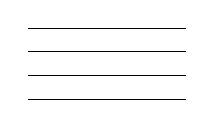
\begin{tikzpicture}
                    \draw (0, 0) -- (2, 0);
                    \draw (0, 0.3) -- (2, 0.3);
                    \draw (0, 0.6) -- (2, 0.6);
                    \draw (0, 0.9) -- (2, 0.9);
                \end{tikzpicture}
                \caption{Unit in $\mathrm{TL}_4(\delta)$.}
                \label{fig:unit_temperley_lieb}
            \end{subfigure}
            \begin{subfigure}{0.49\textwidth}
                \centering
                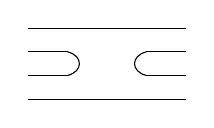
\begin{tikzpicture}
                    \draw (0, 0) -- (2, 0);
                    \draw (0, 0.3) -- (0.5, 0.3);
                    \draw (0, 0.6) -- (0.5, 0.6);
                    \draw (0.5, 0.3) .. controls (0.7, 0.35) and (0.7, 0.55) .. (0.5, 0.6);
                    \draw (1.5, 0.3) -- (2, 0.3);
                    \draw (1.5, 0.6) -- (2, 0.6);
                    \draw (1.5, 0.3) .. controls (1.3, 0.35) and (1.3, 0.55) .. (1.5, 0.6);
                    \draw (0, 0.9) -- (2, 0.9);
                \end{tikzpicture}
                \caption{Generator $U_2$ in $\mathrm{TL}_4(\delta)$.}
                \label{fig:generator_temperley_lieb}
            \end{subfigure}
            \caption{Temperley-Lieb algebra.}
        \end{figure}
    \end{example}

    \newdef{Jordan algebra}{\index{Jordan!algebra}\label{linalgebra:jordan_algebra}
        A nonassociative, commutative algebra $A$ such that
        \begin{gather}
            (xy)(xx) = x(y(xx))
        \end{gather}
        for all $x,y\in A$.
    }
    \begin{property}[Power associativity]
        It can be shown that the Jordan condition implies that powers of elements are well-defined:
        \begin{gather}
            (xx)x = x(xx) =: x^3
        \end{gather}
        for all $x\in A$ and likeiwse for higher-order powers.
    \end{property}

    The original definition of a Jordan algebra does not admit a lot of intuition. However, by the power-associativity property one also has expressions of the form
    \begin{gather}
        (x^my)x^n = x^m(yx^n).
    \end{gather}
    By commutativity one obtains that the multiplication maps $L_{x^m}:y\mapsto x^my$ associated to powers commute:
    \begin{gather}
        \label{linalgebra:power_commuting}
        L_{x^m}L_{x^n} = L_{x^n}L_{x^m}.
    \end{gather}
    This leads to the following equivalent definition:
    \begin{adefinition}
        A Jordan algebra is a commutative, power-associative algebra $A$ such that Equation \eqref{linalgebra:power_commuting} holds for all $x\in A$.
    \end{adefinition}

    \begin{property}
        Every associative algebra over a field of characteristic not 2 (or over a ring in which 2 is a unit) the multiplication induces a Jordan structure as follows:
        \begin{gather}
            x\circ y := \frac{1}{2}(xy+yx),
        \end{gather}
        i.e. the Jordan product is given by the anticommutator. Jordan algebras of this form are said to be \textbf{special}, while all other Jordan algebras are said to be \textbf{exceptional}.
    \end{property}

\section{Grassmanians}

    \newdef{Grassmannian}{\index{Grassmannian}\label{linalgebra:grassmannian}
        Let $V$ be a vector space. The set of all subspaces of $V$ of dimension $k$ is called the Grassmannian $\mathrm{Gr}(k,V)$.
    }
    \begin{property}\label{linalgebra:grassmannian_construction}
        $\GL(V)$ acts transitively \ref{group:transitive} on the $k$-dimensional subspaces of $V$. Property \ref{group:transitive_action_property} implies that the coset space $\GL(V)/H_W$ for the stabilizer $H_W$ of any $W\in\mathrm{Gr}(k,V)$ is isomorphic (as a set) to $\mathrm{Gr}(k,V)$. When $V$ is an $n$-dimensional real vector space one can show that this quotient is isomorphic to $\mathrm{O}(n)/(\mathrm{O}(k)\times\mathrm{O}(n-k))$. For complex vector spaces the orthogonal groups should be replaced by unitary groups.
    \end{property}

    \begin{example}[Projective space]
        Recall Definition \ref{alggeom:projective_space}. The Grassmannian $\mathrm{Gr}(1,V)$ is given by the projective space $K\mathbb{P}^{\dim(V)-1}$.
    \end{example}

    \newdef{Flag}{\index{flag}\index{signature}
        Let $V$ be a finite-dimensional vector space. A sequence of proper subspaces $V_1<\cdots<V_n=V$ is called a flag of $V$. The sequence $(\dim(V_1),\ldots,\dim(V_n)=\dim(V))$ is called the \textbf{signature} of the flag. If $\forall i\leq\dim(V):\dim(V_i) = i$, the flag is said to be \textbf{complete}.
    }

    Grassmannians are a specific instance of the following object:
    \newdef{Flag variety}{\label{linalgebra:flag_manifold}
        The set of all flags of a given signature is called the (generalized) flag variety (of that signature). If the underlying field is the field of real (or complex) numbers, the flag variety is a smooth (or complex) manifold (Chapter \ref{chapter:manifolds}), called the \textbf{flag manifold}.
    }

    Property \ref{linalgebra:grassmannian_construction} generalizes as follows:
    \begin{property}[Parabolic subgroups]\index{para-!bolic subgroup}\index{Borel!subgroup}
        Every flag variety has the structure of a homogeneous space: $\mathrm{Fl}_{n,\underline{d}}=\GL(V)/P_{n,\underline{d}}$, where $\underline{d}$ denotes the signature of the flags. The subgroups $P_{n,\underline{d}}$ are called \textbf{parabolic subgroups}. The maximal parabolic subgroups are those that define the Grassmannian variaties. The flag variety of all complete flags defines the \textbf{Borel subgroup} $B_n$. It can be shown that every parabolic subgroup contains the Borel subgroup.
    \end{property}